\usetikzlibrary{shapes,arrows}
\tikzstyle{ann} = [fill=white,font=\footnotesize,inner sep=1pt]
\tikzstyle{block} = [draw, fill=blue!20, rectangle, 
    minimum height=2.5em, minimum width=3em]
\tikzstyle{circle} = [draw, fill=blue!20, ellipse, 
    minimum height=0.75em, minimum width=0.75em]
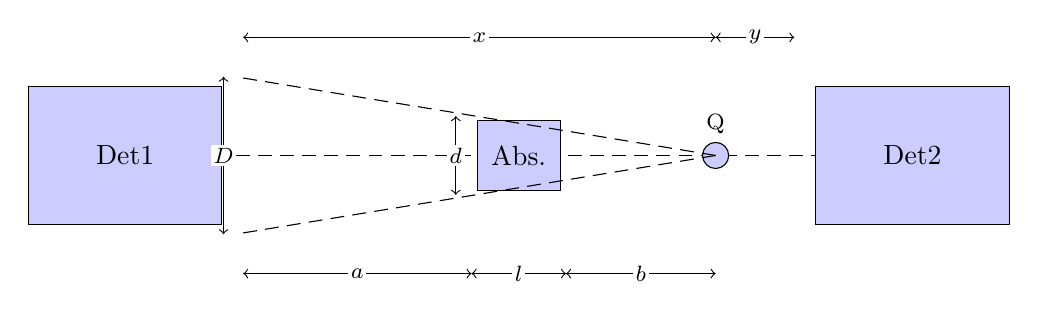
\begin{tikzpicture}
 \coordinate (L) at (-5,0);
 \coordinate (R) at (5,0);
\coordinate (A) at (2.5,4.3);
\coordinate (O) at (2.5,0);

\draw[dash pattern=on5pt off3pt] (L) -- (R);


\node[block, name=det1, minimum height=5em, minimum width=7em] at (L) {Det1};
\node[block, name=det2, minimum height=5em, minimum width=7em, rotate=0] at (R) {Det2};
\node[circle, name=source] at (O) {};
\node[block, name=absorber] at (-0,0){Abs.};

\draw[dash pattern=on5pt off3pt] (O) -- (-3.6,1);
\draw[dash pattern=on5pt off3pt] (O) -- (-3.6,-1);

\draw[arrows=<->](-3.75,1)--(-3.75,-1);
\node[ann] at (-3.75,0) {$D$};

\draw[arrows=<->](-3.5,-1.5)--(-0.6,-1.5);
\node[ann] at (-2.05,-1.5) {$a$};

\draw[arrows=<->](0.6,-1.5)--(-0.6,-1.5);
\node[ann] at (0,-1.5) {$l$};

\draw[arrows=<->](0.6,-1.5)--(2.5,-1.5);
\node[ann] at (1.55,-1.5) {$b$};

\draw[arrows=<->](-0.8,-0.5)--(-0.8,0.5);
\node[ann] at (-0.8,0) {$d$};

\draw[arrows=<->](-3.5,1.5)--(2.5,1.5);
\node[ann] at (-0.5,1.5) {$x$};

\draw[arrows=<->](3.5,1.5)--(2.5,1.5);
\node[ann] at (3,1.5) {$y$};

\node[ann] at (2.5,0.4) {Q};




\end{tikzpicture}